% \documentclass[10pt, headsepline, captions=tableabove, xcolor=table]{beamer}
\documentclass[10pt, handout, headsepline, captions=tableabove, xcolor=table]{beamer}   
% to print 4 in one page

% \makeatletter
% % A new section definition to automatically set labels with the name: sec:sectionnumber
% \let\oldsection\section
% \renewcommand{\section}[1]{\oldsection{#1}\label{sec:\thesection}}
% % A new subsection definition to automatically set labels with the name: sec:sectionnumber.subsectionnumer
% \let\oldsubsection\subsection
% \renewcommand{\subsection}[1]{\oldsubsection{#1}\label{sec:\thesection.\thesubsection}}
% %init some calculators
% \newcounter{calculator}
% \newcounter{calcmaxsec}
% \newcounter{calcmaxsubsec}
% \newcommand{\calcsubsection}[1]%procedure to get the name of section thissection+i
% {
%     \setcounter{calculator}{\thesubsection}\addtocounter{calculator}{#1}
%     \@ifundefined{r@sec:\thesection.\thecalculator}{}{\color{fg!40!bg}\nameref{sec:\thesection.\thecalculator}}
% }
% \newcommand{\calcsection}[1]%procedure to get the name of subsection thissection.thissubsection+i
% {
%     \setcounter{calculator}{\thesection}\addtocounter{calculator}{#1}
%     \@ifundefined{r@sec:\thesection}{}{\color{fg!40!bg}\nameref{sec:\thecalculator}}
% }
% \newcommand{\Testframe}%some testframe definition
%     {
%         \begin{frame}
%             The Section: \thesection\\
%             The Subsection: \thesubsection\\
%             The Calculator: \thecalculator\\
%             Count\thesection
%         \end{frame}
%     }
% %Defining the layout%%%%%%%%%%%%%%%%%%%%%%%%%%%
% \setbeamertemplate{headline}
% {%
%   \leavevmode%
%   \@tempdimb=2.4375ex%
%   \ifnum\beamer@subsectionmax<\beamer@sectionmax%
%      \multiply\@tempdimb by\beamer@sectionmax%
%   \else%
%      \multiply\@tempdimb by\beamer@subsectionmax%
%   \fi%
%   \ifdim\@tempdimb>0pt%
%      \advance\@tempdimb by 1.125ex%
%      \begin{beamercolorbox}[wd=.5\paperwidth,ht=\@tempdimb,right,rightskip=1em]{section in head/foot}%
%         \vbox to \@tempdimb{%
%         \setcounter{calcmaxsec}{\thesection}\addtocounter{calcmaxsec}{-\beamer@sectionmax}
%         \ifnum\thecalcmaxsec>-1\vfill{\calcsection{-3}}\fi%
%         \ifnum\thecalcmaxsec>-2\vfill{\calcsection{-2}}\fi%
%         \ifnum\thesection>1\vfill{\calcsection{-1}}\fi%
%         \ifnum\thesection>0\vfill\insertsectionhead\fi
%         \ifnum\thecalcmaxsec<0\vfill{\calcsection{1}}\fi
%         \ifnum\thecalcmaxsec<-1\vfill{\calcsection{2}}\fi
%         \ifnum\thesection<2\vfill{\calcsection{3}}\fi
%         \ifnum\thesection<1\vfill{\calcsection{4}}\fi
%         \vfill%
%      }%
%      \end{beamercolorbox}%
%      \begin{beamercolorbox}[wd=.5\paperwidth,ht=\@tempdimb]{subsection in head/foot}%
%         \vbox to \@tempdimb{%
%         \setcounter{calcmaxsubsec}{\thesubsection}\addtocounter{calcmaxsubsec}{-\beamer@subsectionmax}
%         \ifnum\thecalcmaxsubsec>-1 \vfill{\calcsubsection{-3}}\fi%
%         \ifnum\thecalcmaxsubsec>-2 \vfill{\calcsubsection{-2}}\fi%
%         \ifnum\thesubsection>1 \vfill{\calcsubsection{-1}}\fi%
%         \ifnum\thesubsection>0 \vfill\insertsubsectionhead\fi
%         \ifnum\beamer@subsectionmax>1{\ifnum\thecalcmaxsubsec<0\vfill{\calcsubsection{1}}\fi}\fi
%         \ifnum\beamer@subsectionmax>2{\ifnum\thecalcmaxsubsec<-1\vfill{\calcsubsection{2}}\fi}\fi
%         \ifnum\beamer@subsectionmax>3{\ifnum\thesubsection<2\vfill{\calcsubsection{3}}\fi}\fi
%         \ifnum\beamer@subsectionmax>4{\ifnum\thesubsection<1\vfill{\calcsubsection{4}}\fi}\fi
%         \vfill%
%       }%
%      \end{beamercolorbox}%
%   \fi%
% }%
% \makeatother %%%%%%%%%%%%%%%%%%%%%%

\usepackage{totcount}
\newcounter{totalsection}
\regtotcounter{totalsection}

\AtBeginDocument{%
  \pretocmd{\section}{\refstepcounter{totalsection}}{}{}%
}%

% number of subsections per section %%%%%%%%%%%%%%%%%%%%%%%%%%%%%%%%%%
\usepackage{xcntperchap}
\RegisterCounters{section}{subsection}
\newcounter{totalsubsection}
\setcounter{totalsubsection}{0}




\newcounter{currentsub}
\setcounter{currentsub}{0}
\newcounter{totsection}
\AtBeginSection[]{%
    \setcounter{currentsub}{\ObtainTrackedValueExp[\thesection]{section}{subsection}}
    \recalc
}

\makeatletter
\setbeamertemplate{headline}{%
  \leavevmode%
  \@tempdimb=2.4375ex%
  \ifnum\thecurrentsub<\beamer@sectionmax%
    \multiply\@tempdimb by\beamer@sectionmax%
  \else%
    \multiply\@tempdimb by\thecurrentsub%
  \fi%
  \ifdim\@tempdimb>0pt%
    \advance\@tempdimb by 1.825ex%
    \begin{beamercolorbox}[wd=.5\paperwidth,ht=\@tempdimb]{section in head/foot}%
      \vbox to\@tempdimb{\vfil\insertsectionnavigation{.5\paperwidth}\vfil}%
    \end{beamercolorbox}%
    \begin{beamercolorbox}[wd=.5\paperwidth,ht=\@tempdimb]{subsection in head/foot}%
      \vbox to\@tempdimb{\vfil\insertsubsectionnavigation{.5\paperwidth}\vfil}%
    \end{beamercolorbox}%
  \fi%
}

\newcommand{\recalc}{\beamer@calculateheadfoot}
\makeatother
\title{Lógica Matemática}
\subtitle{Parte 2}
\author[Paulo Pinheiro]
{Dr. Paulo Vinicius Pereira Pinheiro\inst{1}}
\institute[UNIFAP]
{
    \inst{1}
    Centro Universitário Paraíso do Ceará\\
    UNIFAP
}
%
\date{\small{Acesse estes slides em:\\ \url{https://github.com/paulovpp/slides}}\newline \\Última atualização:\\ \today}
% \logo{
\includegraphics[height=0.7cm]{imgs/UNIFAP.png}}
%

%
\begin{document}
% Delete this, if you do not want the table of contents to pop up at
% the beginning of each subsection:
% \AtBeginSubsection[]
% {
% 	\begin{frame}<beamer>{Sumário do capítulo}
% 		% \tableofcontents[currentsection,currentsubsection]
% 		% \tableofcontents[currentsection, hideothersubsections,sectionstyle=show/shaded,]
%         \tableofcontents[sectionstyle=show/hide,subsectionstyle=show/show/hide]
% 	\end{frame}
% }


% \setcounter{tocdepth}{1} % Show sections
% \setcounter{tocdepth}{2} % + subsections
% Title page frame
\begin{frame}
    \begin{tikzpicture}[remember picture,overlay]
        \node[above right, inner xsep=0pt, inner ysep=20pt] at (current page.south west)
        {
            
\includegraphics[width=\paperwidth]{back36.png}
        };
    \end{tikzpicture}
    \titlepage
    \tikz [remember picture, overlay] %
    \node [shift={(0.1cm,1.4cm)}] at (current page.south west) %
    [anchor=north west] %
    {
\includegraphics[height=0.9cm]{UNIFAP.png}};
\end{frame}

% Remove logo from the next slides
\logo{}

% Outline frame
\begin{frame}[t]{Sumário}
    \begin{tikzpicture}[remember picture,overlay]
        \node[above right, inner xsep=0pt, inner ysep=40pt] at (current page.south west)
        {
            
\includegraphics[width=\paperwidth]{top-right.png}
        };
    \end{tikzpicture}
    \tableofcontents[sections={1-3}]
\end{frame}
%
\begin{frame}[t]{Sumário}
    \begin{tikzpicture}[remember picture,overlay]
        \node[above right, inner xsep=0pt, inner ysep=40pt] at (current page.south west)
        {
            
\includegraphics[width=\paperwidth]{top-right.png}
        };
    \end{tikzpicture}
    \tableofcontents[sections={4-}]
\end{frame}

% \begin{frame}[t]{Sumário}
%     \tableofcontents[sections={4-}]
% \end{frame}

%% -------------------------------- %% -----------------------------------%%
%% Section 1 - Introductory concepts
%% Section 1 - Tabela verdade
\section{Tabela verdade}
%
\subsection{Definições iniciais}
%
\begin{frame}[c]
    \frametitle{Definições iniciais}
    \framesubtitle{Introductory definitions to the topic}
    \begin{block}{Número de linhas}
        O número de linhas de uma tabela verdade de uma proposição composta depende do número $n$ de proposições simples que a integram sendo dado pela regra: \\[2pt]
        \begin{equation}
            2^n \quad \text{linhas}
        \end{equation}
    \end{block}
    %
    \begin{tcolorbox}[colback=red!5,colframe=red!75!black,title=My title]
        My cool formalization
        \tcblower
        \begin{equation}
            \displaystyle\sum\limits_{i=1}^n i = \frac{n(n+1)}{2}    
        \end{equation}
        \textcolor{red}{Text in RED!!}
    \end{tcolorbox}
\end{frame}
%
\subsection{Construção de uma tabela verdade}
%
{
\setbeamercolor{background canvas}{bg=black!15!white}
\begin{frame}[t]
    \frametitle{Construção de uma tabela verdade}
    \framesubtitle{True table construction}
    %
    \begin{exampleblock}{Estudo de caso}
        Caso 1: $H(p,q) = \lnot (p~\land \lnot q)$
    \end{exampleblock}
    %
    \begin{table}[T]
        \caption{Composição de tabela verdade.}
        \label{tab:tabela-caso-1}
        \begin{tabular}{|c|c|c|l|l|}
            % \tiny
            \hline
            \rowcolor[HTML]{EFEFEF} 
            \textbf{p} & \textbf{q} & \textbf{$\lnot q$} & \textbf{$p~\land \lnot q$} & \textbf{$\lnot (p~\land \lnot q)$} \\ \hline
            $V$ & $V$ &  &  &  \\ \hline
            $V$ & $F$ &  &  &  \\ \hline
            $F$ & $V$ &  &  &  \\ \hline
            $F$ & $F$ &  &  &  \\ \hline
        \end{tabular}
    \end{table}
\end{frame}
}
%
\begin{frame}[t]
    \frametitle{Construção de uma tabela verdade}
    \framesubtitle{True table construction}
    %
    \begin{exampleblock}{Estudo de caso}
        Caso 2: $G(p,q) = \lnot (p~\land \lnot q) \lor \lnot (q~\leftrightarrow p)$
    \end{exampleblock}
    %
    % \vspace{-4mm}
    % \hspace{-10mm}
    %
    \begin{table}[ht]
        \footnotesize
        \caption{Composição de tabela verdade.}
        \label{tab:tabela-caso-2}
        \begin{tabular}{|c|c|c|l|l|l|l|}
            \hline
            \rowcolor[HTML]{EFEFEF} 
            \textbf{p} &
            \textbf{q} &
            \textbf{$p~\land \lnot q$} &
            \textbf{$q \leftrightarrow p$} &
            \textbf{$\lnot (p~\land \lnot q)$} &
            \textbf{$\lnot (q \leftrightarrow p)$} &
            \textbf{$\lnot (p~\land q) \lor \lnot (q~\leftrightarrow p)$} \\ \hline
            $V$ & $V$ &  &  &  &  &  \\ \hline
            $V$ & $F$ &  &  &  &  &  \\ \hline
            $F$ & $V$ &  &  &  &  &  \\ \hline
            $F$ & $F$ &  &  &  &  &  \\ \hline
        \end{tabular}
    \end{table}
\end{frame}
%
%% -------------------------------- %% -----------------------------------%%
%% Section 2 - Propositional logic - beginning
%% Section 2 - Mundo da lógica proposicional
\section{Lógica proposicional - sintaxe e semântica}
%
\subsection{Mundo da lógica proposicional}
%
\begin{frame}[c]
    \setbeamercolor{part title}{fg=white, bg=blue!65!black}
    \begin{beamercolorbox}[rounded=true,shadow=true,sep=12pt,center]{part title}
        \usebeamerfont{section title}\insertsection\par
    \end{beamercolorbox}
\end{frame}
%
\begin{frame}[t]
    \frametitle{Algumas definições}
    \framesubtitle{Some definitions to the topic}
    %
    \begin{tcolorbox}[colback=blue!5,colframe=blue!60!black,adjusted title=Mundo lógico]
        O mundo da lógica conforme conhecemos pode ser dividido em duas partes distintas a seguir:
        \begin{itemize}
            \item Sintaxe - mundo sintático
            \item Semântica - mundo semântico
        \end{itemize}
    \end{tcolorbox}
    %    
    \begin{tcolorbox}[colback=red!5!white,colframe=red!75!black,title=Descritivo]
        \textbf{Sintaxe:} responsável pelo conjunto de símbolos (ALFABETO), conectivos e figuras utilizados pela lógica.
        %
        \tcblower
        %
        \textbf{Semântica:} responsável pelas operações e regras de forma a utilizar da melhor forma possível o conjunto de símbolos.
    \end{tcolorbox}
\end{frame}
%
\begin{frame}[t]
    \frametitle{Algumas definições}
    \framesubtitle{Some definitions to the topic}
    %
    \begin{block}{Na prática}
        \begin{itemize}
            \item O computador é um aparelho extremamente sintático - opera com a representação de símbolos em linguagem de máquina, \textbf{baixo nível} e com a possibilidade de conversão dos mesmos para um nível inteligível aos seres humanos, conhecido como \textbf{alto nível}.
            \item Para que o computador possa desempenhar suas funções, um conjunto de regras (ALGORITMO) precisa ser definido, enviado e traduzido para sua interpretação e execução.
        \end{itemize}
    \end{block}
    %
    \setbeamercolor{block title}{use=structure,fg=black,bg=yellow!75!black}
    \begin{block}{Regras ou significados}
        Caso a definição ou o significado de um conjunto de símbolos não seja bem definido, falhas de semântica podem ocorrer. Isso não fará com que não haja processamento. Porém, o resultado pode não ser o esperado.
    \end{block}
\end{frame}
%
\begin{frame}[t]
    \frametitle{Algumas definições}
    \framesubtitle{Some definitions to the topic}
    %
    \begin{block}{Exemplo de falha semântica}
        Observe o seguinte conjunto de caracteres - símbolos sintáticos:
        \begin{center}
            \textbf{R  E  D  E}
        \end{center}
    \end{block}
        %
    \begin{exampleblock}{}
        \indent Caso o uso do seguinte conjunto de símbolos seja utilizado sem a prévia e correta definição de sua usabilidade, poderá haver uma falha de execução e resultados discrepantes. Observa-se pelo menos três possíveis usos da palavra acima:
        \begin{itemize}
            \item objeto usado para dormir.
            \item objeto usado para pescar.
            \item descrição de um conjunto de computadores.
        \end{itemize}
    \end{exampleblock}
\end{frame}
%
\subsection{Valor lógico de uma proposição composta}
%
\begin{frame}[t]
    \frametitle{Valor lógico de uma proposição composta}
    \framesubtitle{Logical values (interpretations) for compound propositions}
    %
    \begin{tcolorbox}[colback=red!5!white,colframe=red!75!black,title=Definição]
        \indent Dado uma proposição composta $H(p,q, r, \dots)$ pode-se determinar seu valor lógico, V ou F, quando são conhecidos os valores lógicos de suas proposições simples respectivamente.
        %
        \tcblower
        %
        \textbf{Exemplo 1:}
        \begin{tcolorbox}
            Assumindo $P(p,q) = (p \rar q) \rar (p \rar p\e q)$, calcule: \\
            $V(P)$ quando $V(p)=V(q)=F$: \\ [4pt]
            $V(P(F,F))=V(P)=(F \rar F) \rar (F \rar F\e F)$ \\
            $V(P)=V \rar (F \rar F)$ \\
            $V(P) = V$
        \end{tcolorbox}
    \end{tcolorbox}
\end{frame}
%
\begin{frame}[t]
    \frametitle{Valor lógico de uma proposição composta}
    \framesubtitle{Logical values (interpretations) for compound propositions}
    %
    \begin{tcolorbox}[colback=red!5!white,colframe=red!75!black,title=Definição]
        \textbf{Exemplo 2:}
        \begin{tcolorbox}
            \vspace{-2pt}
            Dado:
            \vspace{-2pt}
            $$P(p,q,r) = (q \lr (r \rar \n p)) \ou ((\n q \rar p) \lr r)$$
            Calcule $V(P)$ quando $V(p)=V$ e $V(q)=V(r)=F$. \\ [4pt]
            $V(P(VFF)) = (F \lr (F \rar \n V)) \ou ((\n F \rar V) \lr F)$ \\
            $V(P) = (F \lr (F \rar F)) \ou ((V \rar V) \lr F)$ \\
            $V(P) = (F \lr V) \ou (V \lr F)$ \\
            $V(P) = (F) \ou (F)$ \\
            $V(P) = F$
        \end{tcolorbox}
    \end{tcolorbox}
\end{frame}
%
\subsection{Uso de parêntesis}
%
\begin{frame}[t]
    \frametitle{Uso de parêntesis}
    \framesubtitle{Parentheses use}
    %
    \setbeamercolor{block title}{use=structure,fg=white,bg=black!75!black}
    \setbeamercolor{enumerate item}{fg=red!80!black}
    \setbeamertemplate{enumerate items}[default]
    \begin{block}{Definição}
        \indent É óbvia a necessidade do uso dos parêntesis na simbolização das proposições e fórmulas. Muito utilizados para evitar qualquer tipo de ambiguidade. Assim, p. ex., a expressão $p \e q \ou r$ dá lugar, colocando parêntesis, às duas proposições a seguir:
        
        \begin{center}
            (i) $(p \e q) \ou r$ \quad e \quad (ii) $p \e (q \ou r)$
        \end{center}

        \indent Percebe-se aqui que ambas não possuem o mesmo significado pois para ambos os casos os conectivos principais são diferentes. \\ [4pt]
        \indent A supressão de parêntesis nas proposições se faz mediante algumas \textbf{convenções}, mostradas a seguir:
        \begin{enumerate}[\bf I. ]
            \item "A ordem de precedência" para os conectivos.
            \vspace{-2mm}
            $$(1) \sim  \quad (2) \e \ou  \quad (3) \rar \quad (4) \lr$$
        \end{enumerate} 
    \end{block}
\end{frame}
%
\begin{frame}[t]
    \frametitle{Uso de parêntesis}
    \framesubtitle{Parentheses use}
    %
    \setbeamercolor{block title}{use=structure,fg=white,bg=black!75!black}
    \setbeamercolor{enumerate item}{fg=red!80!black}
    \setbeamertemplate{enumerate items}[default]
    \begin{block}{Definição}
        \indent O conectivo mais fraco é, portanto o $\n$. E o mais forte $\lr$. Para o caso abaixo:
        $$ p \rar q \lr s \e r $$
        \indent Temos então uma \textcolor{red}{BICONDICIONAL} e nunca uma condicional. Para convertê-la em uma condicional, o uso dos parêntesis se faz necessário:
        $$ p \rar (q \lr s \e r) $$
        \begin{enumerate}[\bf II. ]
            \item Quando um mesmo conectivo aparece sucessivamente repetido, suprimem-se os parêntesis, fazendo-se a \textbf{associação} a partir da esquerda. Observe as seguintes proposições:
        \end{enumerate} 
    \end{block}
\end{frame}
%
%
\begin{frame}[t]
    \frametitle{Uso de parêntesis}
    \framesubtitle{Parentheses use}
    %
    \setbeamercolor{enumerate item}{fg=red!80!black}
    \setbeamertemplate{enumerate items}[default]
    \begin{exampleblock}{Exemplos}
        \begin{enumerate}[\bf 1.]
            \item $((\n (\n(p \e q))) \ou (\n p))$ \qquad $\longrightarrow$ \qquad $\n \n (p \e q) \ou \n p$
            \vspace{2mm}
            \item $(((p \e (\n q)) \ou r) \e (\n p))$ \qquad $\longrightarrow$ \qquad $(p \ou \n q) \e r \e \n p$
            \vspace{2mm}
            \item $((p \ou (\n q)) \e (r \e (\n p)))$ \qquad $\longrightarrow$ \qquad $(p \e \n q) \e (r \e \n p)$
            \vspace{2mm}
            \item $((\n p) \rar (q \rar (\n (p \ou r))))$ \qquad $\longrightarrow$ \qquad $\n p \rar (q \rar \n (p \ou r))$
        \end{enumerate}
    \end{exampleblock}
    %
    \begin{alertblock}{Outros símbolos para os conectivos}
        Também muito utilizado em linguagens de programação:
        \vspace{-2mm}
        \begin{align*}
            &' \sim '                      &     & \text{para negação.}  \\
            &' \centerdot '~\text{e}~'\&'  &     & \text{para conjunção.} \\
            &' \supset '                   &     & \text{(ferradura) para condicional.} 
        \end{align*}
    \end{alertblock}
\end{frame}
%
% Section 3 - Propriedades semânticas 1
\section{Propriedades semânticas 1}
%
\subsection{Tautologia}
%
\begin{frame}[c]
    \setbeamercolor{part title}{fg=white, bg=blue!65!black}
    \begin{beamercolorbox}[rounded=true,shadow=true,sep=12pt,center]{part title}
        \usebeamerfont{section title}\insertsection\par
    \end{beamercolorbox}
\end{frame}
%
\begin{frame}[t]
    \frametitle{Tautologia}
    \framesubtitle{Tautology definitions}
    %
    \begin{tcolorbox}[colback=red!5!white,colframe=red!75!black,title=Definição]
        Dada uma fórmula $H(p,q,r,\dots)$ ela será uma tautologia quando para qualquer valor lógico de suas proposições simples, seu valor lógico será \textbf{sempre} verdadeiro (V). Ou seja:
        $$ \forall V(p,q,r,\dots) \to V(H)=V$$
        %
        \tcblower
        %
        \textbf{Exemplos:}
        \begin{align*}
            &H_1(p)   = p \ou \n p                  &        & H_2(p) = \n (p \e \n p) \\
            &H_3(p,q) = p \ou \n (p \e q)           &        & H_4(p,q) = p \e q \rar (p \lr p) \\
            &H_5(p,q) = p \ou (q \e \n q) \lr p     &        & H_6(p,q,r) = p \e r \rar \n q \ou r
        \end{align*}
    \end{tcolorbox}
\end{frame}
%
\begin{frame}[t]
    \frametitle{Tautologia - Exemplo}
    \framesubtitle{Tautology example}
    %
    \begin{exampleblock}{Exemplo}
        \centering
        $H_6(p,q,r) = p \e r \rar \n q \ou r $
        %
        \vspace{-2mm}
        %
        \begin{table}[t]
            \caption{Tabela verdade para uma proposição $P(p,q,r)$ tautológica.}
            \label{tab:exemple-tautology}
            \begin{tabular}{|c|c|c|c|c|c|c|}
            \hline
            \textbf{p} & \textbf{q} & \textbf{r} & $\n q$ & $p \e r$ & $\n q \ou r$ & $p \e r \rar \n q \ou r$ \\ \hline
            $V$        & $V$        & $V$        & $F$    & $V$      & $V$          & $V$                    \\ \hline
            $V$        & $V$        & $F$        & $F$    & $F$      & $F$          & $V$                    \\ \hline
            $V$        & $F$        & $V$        & $V$    & $V$      & $V$          & $V$                    \\ \hline
            $V$        & $F$        & $F$        & $V$    & $F$      & $V$          & $V$                    \\ \hline
            $F$        & $V$        & $V$        & $F$    & $F$      & $V$          & $V$                    \\ \hline
            $F$        & $V$        & $F$        & $F$    & $F$      & $F$          & $V$                    \\ \hline
            $F$        & $F$        & $V$        & $V$    & $F$      & $V$          & $V$                    \\ \hline
            $F$        & $F$        & $F$        & $V$    & $F$      & $V$          & $V$                    \\ \hline
            \end{tabular}
        \end{table}
    \end{exampleblock}
\end{frame}
%
\subsection{Princípio da substituição para as tautologias}
%
\begin{frame}[t]
    \frametitle{Princípio da substituição para as tautologias}
    \framesubtitle{Tautological replacement principle}
    %
    \begin{tcolorbox}[colback=blue!5,colframe=blue!60!black,adjusted title=Definição]
        \indent Seja $H(p,q,r,\dots)$ uma proposição tautológica qualquer e sejam $P(p,q,r,\dots)$, $Q(p,q,r,\dots)$, $R(p,q,r,\dots)$, ... proposições quaisquer formadas a parir do mesmo conjunto de proposições simples.
        
        \tcblower
        
        Realizando a substituição das proposições compostas $P, Q, R, \dots$ em $H$, a nova proposição $$ H(P,Q,R,\dots)$$ também será uma tautologia quaisquer que sejam as proposições $P, Q, R, \dots$ .
    \end{tcolorbox}
\end{frame}
%
\subsection{Contradição}
%
\begin{frame}[t]
    \frametitle{Contradição}
    \framesubtitle{Contradiction definitions}
    %
    \begin{tcolorbox}[colback=red!5!white,colframe=red!75!black,title=Definição]
        Dada uma fórmula $H(p,q,r,\dots)$ ela será uma contradição quando para qualquer valor lógico de suas proposições simples, seu valor lógico será \textbf{sempre} falso (F). Ou seja:
        $$ \forall V(p,q,r,\dots) \to V(H)=F$$
        As contradições também são conhecidas como proposições contraválidas ou logicamente falsas.
        %
        \tcblower
        %
        \textbf{Exemplos:}
        \vspace{-5pt}
        \begin{align*}
            &H_7(p) = p \e \n p                     &        & H_8(p) = p \lr \n p \\
            &H_9(p,q) = (p \e q) \e \n (p \ou q)    &        & H_{10}(p,q) = \n p \e (p \e \n q)
        \end{align*}
    \end{tcolorbox}
\end{frame}
%
\subsection{Contingência}
%
\begin{frame}[t]
    \frametitle{Contingência}
    \framesubtitle{Contigency definitions}
    %
    \begin{alertblock}{Definição}
        \indent Proposições que não são nem tautológicas ou contraválidas chamam-se necessariamente de contingentes. As mesmas possuem em sua última coluna de sua tabela-verdade os valores lógicos V e F \textbf{pelo menos uma vez}.\\
        \hfill \break
        \indent Elas também são conhecidas como \textbf{proposições indeterminadas}. \\
        {\color{red} \rule{\linewidth}{0.5pt}}
        \textbf{Exemplos:}
        \begin{align*}
            &H_{11}(p) = p \rar \n p                     &        & H_{12}(p,q) = p \ou q \rar p \e p \\
            &H_{13}(p,q) = p \ou q \rar p                &        & H_{14}(p,q) = p \rar (p \rar q \e \n q)
        \end{align*}
    \end{alertblock}
\end{frame}
%
\subsection{Exercícios}
%
\begin{frame}[t]
    \frametitle{Exercícios}
    %
    \begin{exampleblock}{Caracterize a proposição como tautológica, contingente ou contraditória.}
        \begin{equation}
            H_1(p,q) = \n (p \ou q) \rar (p \lr q)
        \end{equation}
    \end{exampleblock}
    %
    \begin{table}[]
        \caption{Tabela verdade para uma proposição $H_1(p,q)$.}
        \label{tab:exercise-21}
        \begin{tabular}{|c|c|c|c|c|c|}
            \hline
            \rowcolor[HTML]{EFEFEF} 
            \textbf{p} & \textbf{q} & $p \ou q$ & $\n (p \ou q) $ & $p \rar q$ & $\n (p \ou q) \rar (p \rar q)$ \\ \hline
            $V$        & $V$        &           &              &            &                                \\ \hline
            $V$        & $F$        &           &              &            &                                \\ \hline
            $F$        & $V$        &           &              &            &                                \\ \hline
            $F$        & $F$        &           &              &            &                                \\ \hline
        \end{tabular}
        \\
        \centering \tiny{Fonte: Filho, E. A Iniciação à lógica matemática. Ed. Nobel. 2002 - Q.1k C.5}
    \end{table}
\end{frame}
%
\begin{frame}[t]
    \frametitle{Exercícios}
    %
    \begin{exampleblock}{Caracterize a proposição como tautológica, contingente ou contraditória.}
        \begin{equation}
            H_2(p,q) = (p \lr q) \e p \rar q
        \end{equation}
    \end{exampleblock}
    %
    \begin{table}[]
        \caption{Tabela verdade para uma proposição $H_2(p,q)$.}
        \label{tab:exercise-22}
        \begin{tabular}{|c|c|c|c|c|}
            \hline
            \rowcolor[HTML]{EFEFEF} 
            \textbf{p} & \textbf{q} & $p \lr q$ & $(p \lr q) \e p$ & $(p \lr q) \e p \rar q$ \\ \hline
            $V$        & $V$        &           &                  &                         \\ \hline
            $V$        & $F$        &           &                  &                         \\ \hline
            $F$        & $V$        &           &                  &                         \\ \hline
            $F$        & $F$        &           &                  &                         \\ \hline
        \end{tabular}
        \\
        \centering \tiny{Fonte: Filho, E. A Iniciação à lógica matemática. Ed. Nobel. 2002 - Q.1l C.5}
    \end{table}
\end{frame}
%
\begin{frame}[t]
    \frametitle{Exercícios}
    %
    \begin{exampleblock}{Caracterize a proposição como tautológica, contingente ou contraditória.}
        \begin{equation}
            H_3(p,q,r) = p \rar (p \ou q) \ou r
        \end{equation}
    \end{exampleblock}
    %
    \vspace{-2mm}
    %
    \begin{table}[]
        \caption{Tabela verdade para uma proposição $H_3(p,q,r)$.}
        \label{tab:exercise-23}
        \begin{tabular}{|c|c|c|c|c|c|}
            \hline
            \rowcolor[HTML]{EFEFEF}
            \textbf{p} & \textbf{q} & \textbf{r} & $p \ou q$ & $(p \ou q) \ou r$ & $ p \rar (p \ou q) \ou r$ \\ \hline
            $V$        & $V$        & $V$        &             &                      &                                \\ \hline
            $V$        & $V$        & $F$        &             &                      &                                \\ \hline
            $V$        & $F$        & $V$        &             &                      &                                \\ \hline
            $V$        & $F$        & $F$        &             &                      &                                \\ \hline
            $F$        & $V$        & $V$        &             &                      &                                \\ \hline
            $F$        & $V$        & $F$        &             &                      &                                \\ \hline
            $F$        & $F$        & $V$        &             &                      &                                \\ \hline
            $F$        & $F$        & $F$        &             &                      &                                \\ \hline
        \end{tabular}
        \\
        \centering \tiny{Fonte: Filho, E. A Iniciação à lógica matemática. Ed. Nobel. 2002 - Q.4g C.5}
    \end{table}
\end{frame}
%
\begin{frame}[t]
    \frametitle{Exercícios}
    %
    \begin{exampleblock}{Caracterize a proposição como tautológica, contingente ou contraditória.}
        \begin{equation}
            H_4(p,q,r) = p \e q \rar (p \lr q \ou r)
        \end{equation}
    \end{exampleblock}
    %
    \vspace{-4mm}
    \begin{table}[]
        \caption{Tabela verdade para uma proposição $H_4(p,q,r)$.}
        \label{tab:exercise-24}
        \begin{tabular}{|c|c|c|c|c|c|c|}
        \hline
        \rowcolor[HTML]{EFEFEF} 
        \textbf{p} & \textbf{q} & \textbf{r} & $p \e q$ & $p \lr q$ & $p \lr q \ou r$ & $p \e q \rar (p \lr q \ou r)$ \\ \hline
        $V$        & $V$        & $V$        &          &           &                 &                               \\ \hline
        $V$        & $V$        & $F$        &          &           &                 &                               \\ \hline
        $V$        & $F$        & $V$        &          &           &                 &                               \\ \hline
        $V$        & $F$        & $F$        &          &           &                 &                               \\ \hline
        $F$        & $V$        & $V$        &          &           &                 &                               \\ \hline
        $F$        & $V$        & $F$        &          &           &                 &                               \\ \hline
        $F$        & $F$        & $V$        &          &           &                 &                               \\ \hline
        $F$        & $F$        & $F$        &          &           &                 &                               \\ \hline
        \end{tabular}
        \\
        \centering \tiny{Fonte: Filho, E. A Iniciação à lógica matemática. Ed. Nobel. 2002 - Q.4h C.5}
        \end{table}
\end{frame}
%% -------------------------------- %% -----------------------------------%%
%% Section 3 - Propositional logic - calculus
%% Section 3 - Propositional logic - calculus

\section{Lógica proposicional - cálculo proposicional}
%
\subsection{Tabela verdade}
%
\begin{frame}[t]
    \frametitle{Tabela verdade}
    \framesubtitle{True table of operators}
    %
    \begin{alertblock}{Definição}
        \small
        Segundo o princípio do \textbf{terceiro excluído}, toda proposição simples $p$ ou composta $H(p,q,...)$ só pode assumir \textbf{valor lógico} igual a \\ [1pt]
        \center{$V$ (verdade - \textit{TRUE}) \qquad ou \qquad  $F$ (falsidade - \textit{FALSE})} \\ [4pt]
        A \textbf{tabela-verdade} sintetiza o resultado de funções lógicas para $n$ proposições.
    \end{alertblock}
    %
    \vspace{-4mm}
    %
    \begin{figure}[c]
        \centering
        \caption{Tabela verdade para um estado(proposição) único.}
        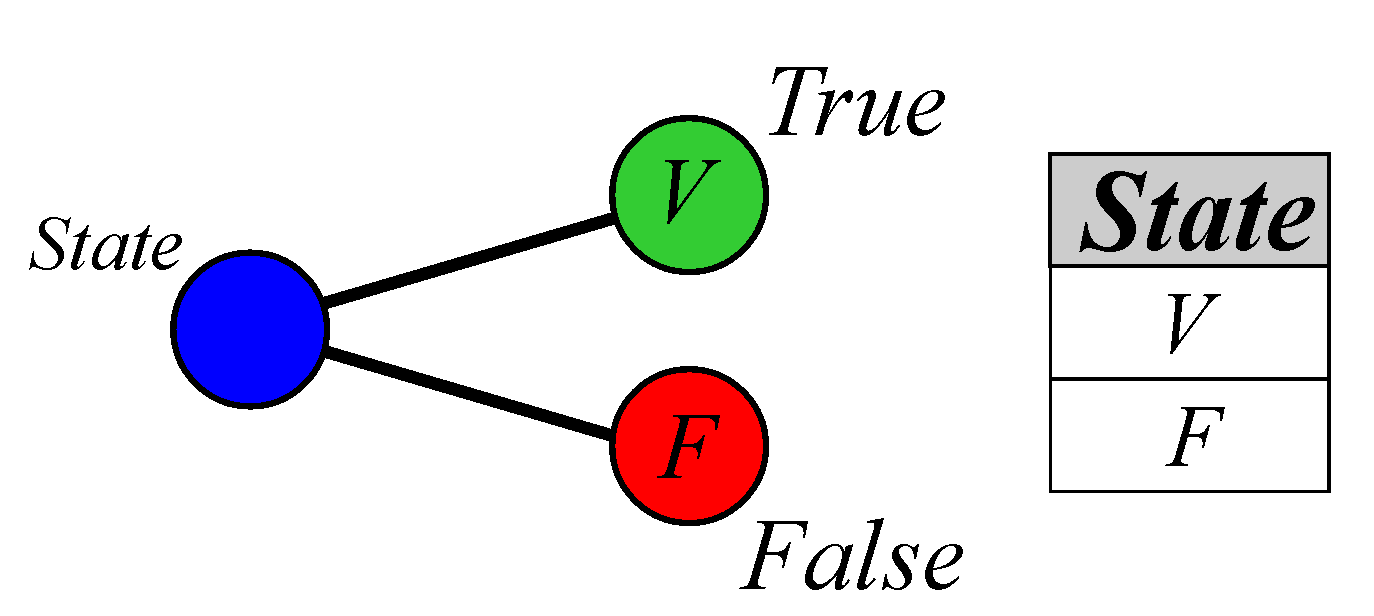
\includegraphics[scale=0.25]{TT2.png}
        \label{fig:tabela-verdade1}         
    \end{figure}
\end{frame}
%
\begin{frame}[c]
    \frametitle{Tabela verdade}
    \framesubtitle{Examples}
    %
    \begin{figure}[c]
        \centering
        \caption{Tabela verdade para uma proposição composta $H(p,q)$.}
        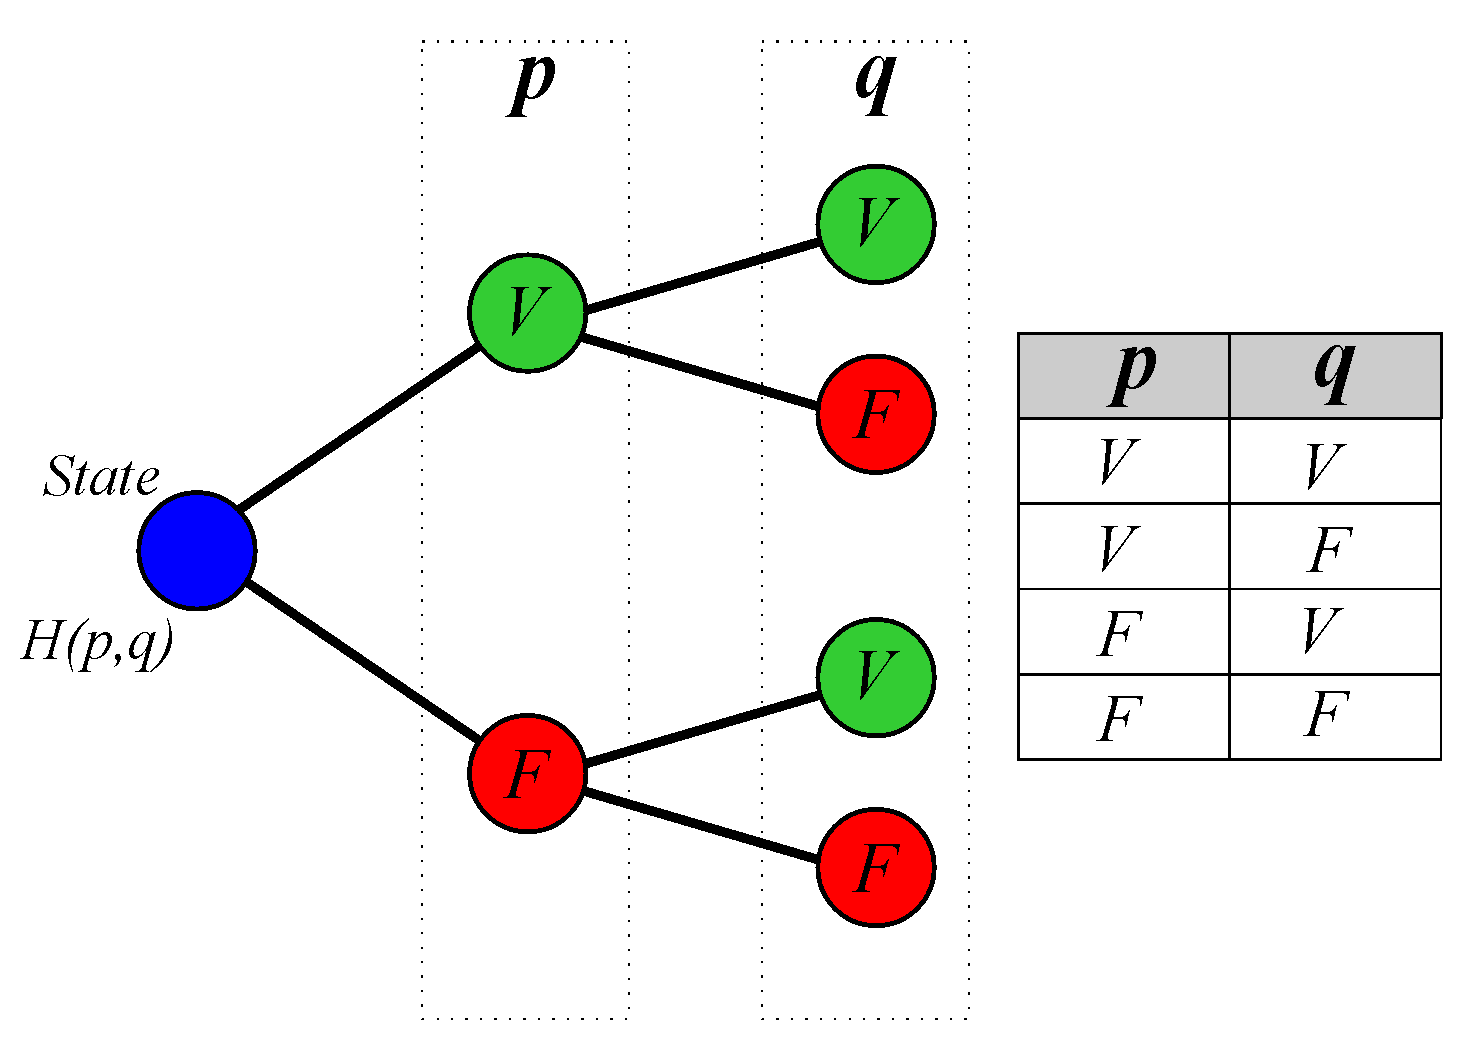
\includegraphics[scale=0.30]{TT3.png}
        \label{fig:tabela-verdade2}
    \end{figure}
\end{frame}
%
\begin{frame}[c]
    \frametitle{Tabela verdade}
    \framesubtitle{Examples}
    %
    \begin{figure}[c]
        \centering
        \caption{Tabela verdade para uma proposição composta $H(p,q,r)$.}
        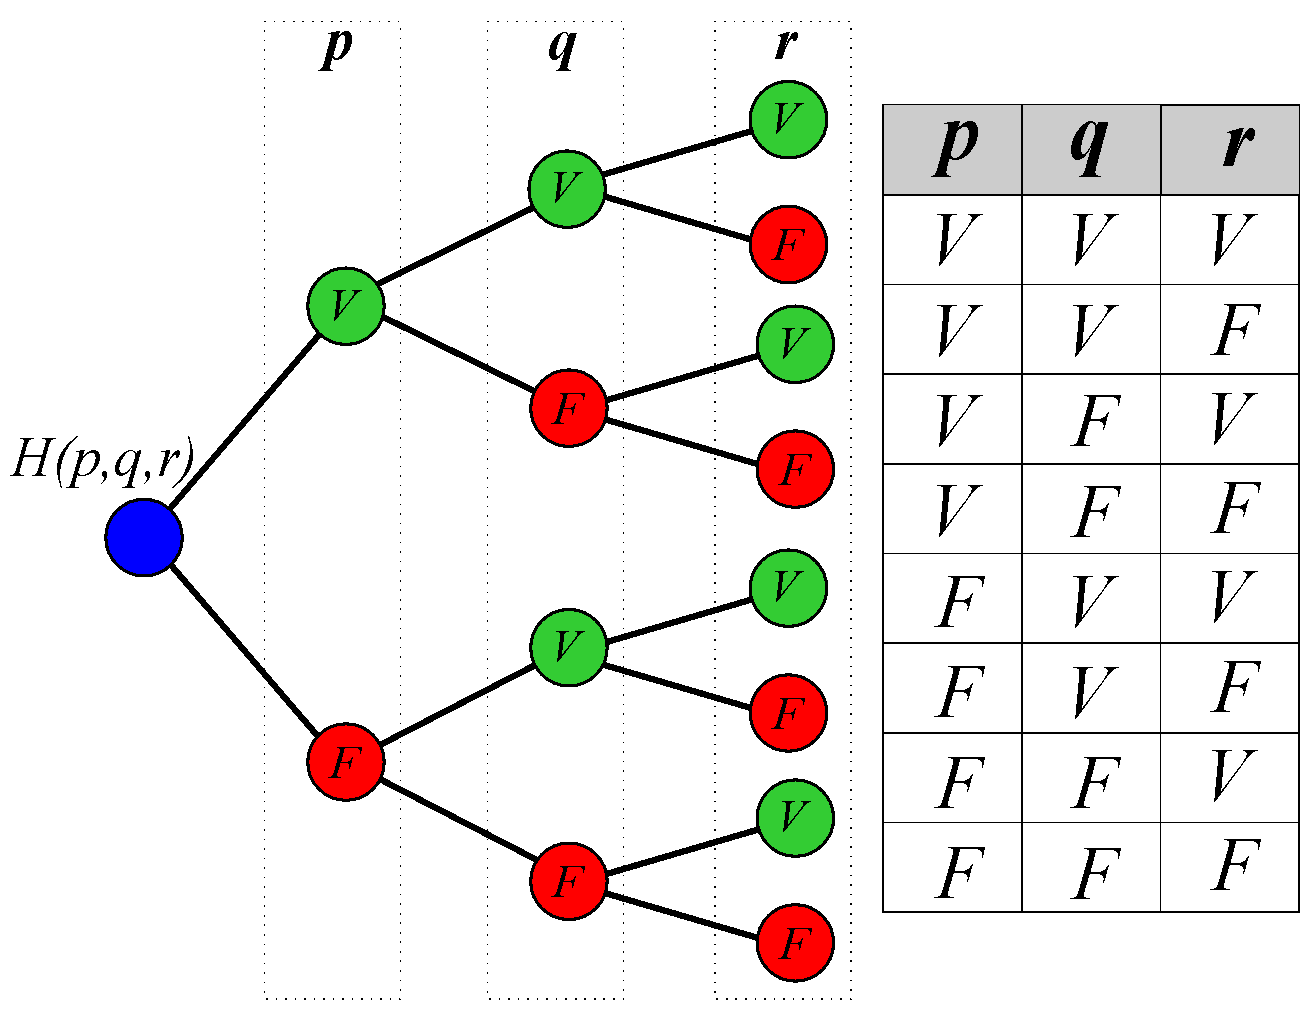
\includegraphics[scale=0.30]{TT4.png}
        \label{fig:tabela-verdade3}
    \end{figure}
\end{frame}
%
\subsection{Ordem de precedência e comprimento de fórmulas}
%
\begin{frame}[t]
    \frametitle{Definições complementares}
    \framesubtitle{Final considerations of the section - Procedence order}
    %
    \small
    \setbeamercolor{block title}{use=structure,fg=white,bg=black!75!black}
    \begin{block}{Ordem de precedência}
        \begin{itemize}
            \item Maior precedência: $\lnot$ ou $\sim$ 
            \item Precedência intermediária: $\rightarrow$ e $\leftrightarrow$
            \item Menor precedência: $\land$ e $\lor$
        \end{itemize}        
    \end{block}
    %
    \pause
    %
    \setbeamercolor{block title}{use=structure,fg=white,bg=orange!75!black}
    \begin{block}{Comprimento de uma fórmula}
        \begin{itemize}
            \item Se $H$ é um símbolo proposicional ou de verdade então $comp[H]=1$
            \item Se $H$ e $G$ são fórmulas da \textbf{lógica proposicional}, então
        \end{itemize}
        %\vspace{-3mm} % if negative it removes vertical space
        \begin{gather*}
            comp[\lnot H] = comp[H] + 1 \\
            comp[H \land G]~\text{ ou }~comp[H \lor G] = comp[H] + comp[G] + 1 \\
            comp[H \rightarrow G]~\text{ ou }~comp[H \leftrightarrow G] = comp[H] + comp[G] + 1
        \end{gather*}
        % gather environment: align equations on center
    \end{block}
\end{frame}
%
\subsection{Valor lógico}
%
\begin{frame}[t]
    \frametitle{Definições finais}
    \framesubtitle{Final considerations of the section 2/2}
    \small
    \begin{block}{Valor lógico}
        O \textbf{valor lógico} de uma proposição simples ou composta expressa seu valor resultante se \textit{verdadeiro} ou \textit{falso}.
        \begin{itemize}
            \item Para uma proposição simples $p$, $V(p)$ expressa seu valor lógico.
            \item Para uma proposição composta $H$, $V(H)$ expressa seu valor lógico.
        \end{itemize}
    \end{block}
        %
    \begin{columns}[T]
        \begin{column}{.5\textwidth}
            \begin{exampleblock}{Exemplo 1}
                \quad $p$ : O sol é verde. \\
                \quad $q$ : O sol é quente. \\
                \quad $r$ : O mar não é vermelho.\\[4pt]
                \quad $V(p) = V$, $V(q) = F$, $V(\lnot r)=F$ \\
                \quad $V(p \land q) = F$, \quad $V(q \lor r) = V$
            \end{exampleblock}
        \end{column}
        %
        %\hspace{5mm}
        \begin{column}{.5\textwidth}
            \begin{exampleblock}{Exemplo 2}
                \quad $p_1$ : $x \geq 10$   \\
                \quad $p_2$ : $x < 50$\\
                \quad $p_3$ : $x > 25$ \\[4pt]
                $V(p_1) = V$, $V(p_2) = F$, $V(\lnot p_3)=F$ \\
                \quad $V(p_1 \land p_2) = V$, $V(p_3 \land p_2) = F$
            \end{exampleblock}
        \end{column}
    \end{columns}
\end{frame}
%
\subsection{Exercícios}
%
\begin{frame}[t] % \renewcommand{\theenumi}{\alph{enumii}}
    \frametitle{Exercícios - 1/2}
    \framesubtitle{Practice the chapters concepts}
    %
    \small
    \setbeamercovered{invisible}
    \setbeamercolor{enumerate item}{fg=red!80!black}
    \setbeamertemplate{enumerate items}[default]
    \begin{exampleblock}{1. Identifique os itens abaixo que não são fórmulas da lógica proposicional.}
        \begin{columns}[T]
            \begin{column}{0.15\textwidth}
                \begin{enumerate}[\bf a.]
                    \item $pq$
                    \item $PQ$
                    \item $PQ \lnot$
                    \item $\lnot PQ$
                \end{enumerate}
            \end{column}
            %
            \hspace*{-5mm}
            %
            \begin{column}{0.15\textwidth}
                \begin{enumerate}[\bf a.]
                    \addtocounter{enumi}{4}
                    \item $p \land q$
                    \item $P \lor Q$
                    \item $PQ \land$
                    \item $\lor PQ$
                \end{enumerate}
            \end{column}
            %
            \hspace*{-5mm}
            %
            \begin{column}{0.20\textwidth}
                \begin{enumerate}[\bf a.]
                    \addtocounter{enumi}{8}
                    \item $p \rightarrow q$
                    \item $PQ \rightarrow$
                    \item $\rightarrow PQ \lnot$
                    \item $P \rightarrow Q \rightarrow $
                \end{enumerate}
            \end{column}
            %
            \hspace*{-7mm}
            %
            \begin{column}{0.2\textwidth}
                \begin{enumerate}[\bf a.]
                    \addtocounter{enumi}{12}
                    \item $P \rightarrow Q$
                    \item $P \leftrightarrow Q$
                    \item $P \leftrightarrow q$
                    \item $\leftrightarrow P \leftrightarrow Q$
                \end{enumerate}
            \end{column}
            %
            \hspace*{-8mm}
            %
            \begin{column}{0.25\textwidth}
                \begin{enumerate}[a.]
                    \addtocounter{enumi}{16}
                    \item $P \rightarrow true$
                    \item $P \land true$
                    \item $true~P \leftrightarrow q$
                    \item $false~PQ \land$
                \end{enumerate}
            \end{column}
        \end{columns}
    \end{exampleblock}
    %
    \pause
    \vspace{-2mm}
    %
    \begin{alertblock}{Respostas}
        a, b, c, d, g, h, j, k, l, p, q, s, t
    \end{alertblock}
    %
    \pause
    \vspace{-2mm}
    %
    % \setbeamercolor{enumerate item}{fg=red!80!black}
    % \setbeamertemplate{enumerate items}[default]
    \begin{exampleblock}{2. Determine o comprimento das fórmulas a seguir.}
        \begin{columns}[T]
            \begin{column}{0.8\textwidth}
                \begin{enumerate}[\bf a.]
                    \item $((\lnot \lnot~P \land Q) \leftrightarrow (P \rightarrow Q)) \land~true$
                    \item $(\lnot P \rightarrow (Q \lor R)) \leftrightarrow ((P \land Q) \leftrightarrow (\lnot \lnot R \lor \lnot P))$
                    \item $((P \lor Q) \rightarrow (P \rightarrow (\lnot Q)))$
                \end{enumerate}
            \end{column}
            %
            \pause
            %
            \begin{column}{0.2\textwidth}
                \begin{enumerate}[\bf a.]
                    \item 11
                    \item 17
                    \item 8
                \end{enumerate}
            \end{column}
        \end{columns}
    \end{exampleblock}
\end{frame}
%
\begin{frame}[t] % \renewcommand{\theenumi}{\alph{enumii}}
    \frametitle{Exercícios - 2/2}
    \framesubtitle{Practice the chapters concepts}
    %
    \small
    \setbeamercolor{enumerate item}{fg=red!80!black}
    \setbeamertemplate{enumerate items}[default]
    \begin{exampleblock}{3. Pesquise na internet as proposições para os problemas abaixo.}
        E, se possível, elabore a fórmula para avaliar um valor qualquer.\\
        \begin{enumerate}[\bf P1.]
            \item Verificar se um número $n \in \mathbb{Z} $ está no intervalo $\{n_1, n_2\}$ onde $n_1 < n_2$.
            \item Descobrir o maior entre 2 números.
            \item Descobrir o maior entre 3 números.
            \item Ordenar 2 números.
            \item Ordenar 3 números.
            \item Avaliar se um número é primo.
            \item Buscar letra em palavra (string).
            \item Transformar um tempo dado em \textbf{HH:mm:ss} em apenas \textbf{ss}.
        \end{enumerate}
    \end{exampleblock}
    %
    \normalsize
    \center{\textcolor{red}{\textbf{Trazer na próxima aula para tira-dúvidas.}}}
    \end{frame}
%%% -------------------------------- %% -----------------------------------%%
% Section 4 - Fundamental operations under logic propositions
% Section 4 - Fundamental operations under logic propositions

\section{Operações lógicas com proposições}
%
\begin{frame}[c]
    \frametitle{Operações lógicas}
    \framesubtitle{Logical operation with propositions}
    %
    \textbf{Operadores da lógica proposicional}\\[2pt]
    \textcolor{green!50!black}{\textbf{Quando pensamos, inerentemente ao processo estamos efetuando inúmeras operações com proposições em nossa mente. Sempre na intenção de formar um raciocínio que nos faça sentido e que possa ser solução para um determinado problema.}}\\[6pt]

    \textcolor{red}{\textbf{As operações lógicas acontecem exatamente com os conectivos proposicionais. Na literatura é comum as duas nomenclaturas se confundirem.}}\\[6pt]
    
    Neste curso, usaremos a notação de \textbf{OPERADORES}. A seguir, as operações lógicas e seus descritivos serão apresentados.

\end{frame}



\subsection{Negação}



\begin{frame}[t]
    \frametitle{Operação de negação $(\lnot)$ ou $(\sim)$}
    \framesubtitle{Logical NOT operator}
    %
    \begin{block}{Definição}
        Este conectivo não liga duas proposições, mas simplesmente nega a afirmação da proposição que o precede. Em virtude disso, é um conectivo unário, enquanto os anteriores são conectivos binários, pois ligam duas proposições.
    \end{block}
    %
    \vspace{-4mm}
    %
    \begin{columns}[t]
        \begin{column}{0.55\textwidth}
            \small
            \begin{exampleblock}{Exemplos}
                Se $V(p) = V$, $\lnot p = F$ \\ [2pt]
                $V(\lnot p) = \lnot V(p)$ \\ [2pt]
                $p:~2+3=5\quad (V)$ e $\lnot p:~2+3 \neq 5\quad (F)$ \\ [2pt]
                $q:~23 < 10 \quad (F)$ e $\lnot q:~23 \nless 10 \quad (V)$ \\[2pt]
                $q:$ Carlos é mecânico. \\[2pt]
                $\lnot q:$ Carlos NÃO é mecânico.
            \end{exampleblock}
        \end{column}
        %
        \hspace{-5mm}
        %
        \begin{column}{0.4\textwidth}
            \vspace{-3mm}
            \begin{table}[t]
                \caption{Tabela verdade $(\lnot)$.}
                \label{tab:tabela-not}
                \begin{tabular}{|c|c|}
                \hline
                \rowcolor[HTML]{EFEFEF} 
                \textbf{$~$p} & \textbf{$\sim$p} \\ \hline
                V          & F                \\ \hline
                F          & V                \\ \hline
                \end{tabular}
            \end{table}
        \end{column}
    \end{columns}
\end{frame}
%
\subsection{Conjunção}
%

\begin{frame}[t]
    \frametitle{Conjunção ($\land$ - 'e' lógico)}
    \framesubtitle{Logical AND operation}
    % 
    \begin{block}{Definição}
        É o resultado da combinação de duas proposições ligadas pela palavra \textbf{e}, que será substituída pelo símbolo $(\land)$. Seu \textbf{valor lógico} somente será VERDADEIRO quando \emph{TODAS} as proposições tiverem seus \textbf{valores lógicos} iguais a VERDADE.
    \end{block}
    %
    \vspace{-4mm}
    %
    \begin{columns}[t]
        \begin{column}{0.58\textwidth}
            \begin{alertblock}{Propriedades}
                Sejam $p$ e $q$ proposições simples: \\[2pt]
                $p \land q$ lê-se "p e q". \\[2pt]
                Seja $H$ uma proposição composta $H(p,q)$: \\[2pt]
                $H(p,q) = H(p \land q) = p \land q$ \\[2pt]
                $V(H) = V(p \land q) = V(p) \land V(q)$
            \end{alertblock}
        \end{column}
        %
        \hspace{-10mm}
        %
        \begin{column}{0.4\textwidth}
            \vspace{-3mm}
            \begin{table}[t]
                \caption{Tabela verdade $(\land)$.}
                \label{tab:table-and}
                \begin{tabular}{|c|c|c|}
                \hline
                \rowcolor[HTML]{EFEFEF} 
                \textbf{p} & \textbf{q} & \textbf{$p \land q$} \\ \hline
                $V$          & $V$          & $V$                    \\ \hline
                $V$          & $F$          & $F$                    \\ \hline
                $F$          & $V$          & $F$                   \\ \hline
                $F$          & $F$          & $F$                    \\ \hline
                \end{tabular}
            \end{table}
        \end{column}
    \end{columns}
\end{frame}
%
\begin{frame}[t]
    \frametitle{Conjunção ($\land$ - 'e' lógico)}
    \framesubtitle{Examples}
    %
    \begin{exampleblock}{Exemplo 1}
        Sejam $p$ e $q$ proposições simples quaisquer, por exemplo:
        \begin{itemize}
            \item $p:~n > 10 \quad (V)$
            \item $q:~f(n) = 55 \quad (V)$
        \end{itemize}
        $p \land q = (n >10)~e~(f(n = 55)) = V$ \\[2pt]
        $V(p \land q) = V(p) \land V(q) = V \land V = V$
    \end{exampleblock}
    %
    % \vspace{-3mm}
    \begin{exampleblock}{Exemplo 2}
        Seja $H(p,q)$ uma proposição composta qualquer, por exemplo:
        \begin{itemize}
            \item $p:$ A maça é vermelha $(V)$
            \item $q:$ A rua é estreita  $(F)$
        \end{itemize}
        $H(p,q) = p \land q = V \land F = F$
    \end{exampleblock}
\end{frame}
%
\subsection{Disjunção}
%
\begin{frame}[t]
    \frametitle{Disjunção ($\lor$ - 'ou' lógico)}
    \framesubtitle{Logical OR operator}
    %
    \begin{block}{Definição}
        É o resultado da combinação de duas proposições ligadas pela palavra \textbf{ou}, que será substituída pelo símbolo $\lor$. Seu \textbf{valor lógico} somente será FALSO quando \emph{TODAS} as proposições tiverem seus \textbf{valores lógicos} iguais a FALSO.
    \end{block}
    %
    \vspace{-4mm}
    %
    \begin{columns}[t]
        \begin{column}{0.55\textwidth}
            \small
            \begin{alertblock}{Propriedades}
                Sejam $p$ e $q$ proposições simples: \\[2pt]
                $p \lor q$ lê-se "p ou q". \\[2pt]
                Seja $H$ uma proposição composta $H(p,q)$: \\[2pt]
                $H(p,q) = H(p \lor q) = p \lor q$ \\[2pt]
                $V(H) = V(p \lor q) = V(p) \lor V(q)$
            \end{alertblock}
        \end{column}
        %
        \hspace{-10mm}
        %
        \begin{column}{0.4\textwidth}
            \vspace{-3mm}
            \begin{table}[ht]
                \caption{Tabela verdade $(\lor)$.}
                \label{tab:my-table}
                \begin{tabular}{|c|c|c|}
                \hline
                \rowcolor[HTML]{EFEFEF} 
                \textbf{p} & \textbf{q} & \textbf{$p\lor q$} \\ \hline
                $V$        & $V$        & $V$                 \\ \hline
                $V$        & $F$        & $V$                 \\ \hline
                $F$        & $V$        & $V$                 \\ \hline
                $F$        & $F$        & $F$                 \\ \hline
                \end{tabular}
            \end{table}
        \end{column}
    \end{columns}
\end{frame}
%
\begin{frame}[t]
    \frametitle{Disjunção ($\lor$ - 'ou' lógico)}
    \framesubtitle{Examples}
    %
    \begin{exampleblock}{Exemplo 1}
        Sejam $p$ e $q$ proposições simples quaisquer, por exemplo:
        \begin{itemize}
            \item $p:~n > 10 \quad (V)$
            \item $q:~n \leq 25 \quad (V)$
        \end{itemize}
        $p \lor q = (n >10)~ou~(n \leq 55) = V$ \\[2pt]
        %$V(p \lor q) = V(p) \lor V(q) = V \lor V = V$
    \end{exampleblock}
    %
    % \vspace{-3mm}
    \begin{exampleblock}{Exemplo 2}
        Seja $H(p,q)$ uma proposição composta qualquer, por exemplo:
        \begin{itemize}
            \item $p:$ Maria foi ao cinema. $(V)$
            \item $q:$ Maria foi ao teatro. $(F)$
        \end{itemize}
        $H(p,q):$ Maria foi ao cinema ou ao teatro. \\[2pt]
        $H(p,q) = p \lor q = V \lor F = F$
    \end{exampleblock}
\end{frame}
%
\subsection{Disjunção exclusiva}
%
\begin{frame}[t]
    \frametitle{Disjunção exclusiva ($\veebar$ - 'ou exclusivo' lógico)}
    \framesubtitle{Logical XOR operator}
    %
    \begin{block}{Definição}
        Na linguagem falada, o termo "ou" tem \textbf{dois significados}. Por exemplo:\\ [2pt]
        $H:$ Antonio é cearense e pernambucano. \\[2pt]
        $G:$ José é eletricista e encanador.
    \end{block}
    %
    \vspace{-2mm}
    \pause
    %
    \begin{block}{}
        Na proposição $H$ existe a indicação de duas proposições:
        \begin{itemize}
            \item[] $p:$ Antonio é cearense.
            \item[] $q:$ Antonio é pernambucano.
        \end{itemize}
        Nota-se pelo contexto que \textbf{APENAS} uma das proposições pode ser verdadeira, tornando assim o resultado \textbf{mutualmente excludente}.
    \end{block}
    %
    \vspace{-2mm}
    \pause
    %
    \begin{block}{}
        Para a proposição compostas $H(p,q)$ têm-se que:
        \begin{itemize}
            \item $H(p,q) = p \veebar q$
        \end{itemize}
    \end{block}
\end{frame}
%
\begin{frame}[t]
    \frametitle{Disjunção exclusiva ($\veebar$ - 'ou exclusivo' lógico)}
    \framesubtitle{Logical XOR operator}
    %
    \vspace{-2mm}
    \begin{block}{Comparativo}
        Já para a proposição $G(r,s) \longrightarrow G(r,s) = r \lor s $:
        \begin{itemize}
            \item[] $r:$ José é eletricista.
            \item[] $s:$ José é encanador.
        \end{itemize}
        Percebe-se então que no caso da proposição $G$, as duas proposições simples $r$ e $s$ não são \textbf{mutualmente excludentes}. Ou seja, ambas podem ter seus \textbf{valores lógicos} iguais a VERDADEIRO. \\[2pt]
    \end{block}
    %
    \vspace{-5mm}
    %
    \begin{table}[ht]
        \caption{Tabela verdade $(\veebar)$.}
        \label{tab:tabela-xor}
        \begin{tabular}{|c|c|c|}
        \hline
        \rowcolor[HTML]{EFEFEF} 
        \textbf{p} & \textbf{q} & \textbf{p $\veebar$ q} \\ \hline
        $V$        & $V$        & $F$                    \\ \hline
        $V$        & $F$        & $V$                    \\ \hline
        $F$        & $V$        & $V$                    \\ \hline
        $F$        & $F$        & $F$                    \\ \hline
        \end{tabular}
    \end{table}
\end{frame}
%%% -------------------------------- %% -----------------------------------%%
% Section 5 - Logical operations with conditions
% Section 5 - Logical operations with conditions

\section{Operações lógicas condicionais}
%
\subsection{Condicional}
%
\begin{frame}[t]
    \frametitle{Operador condicional $(\rightarrow)$ }
    \framesubtitle{Conditional operator}
    %
    \vspace{-2mm}
    \begin{block}{Definição}
        Duas proposições formam uma condicional quando for possível colocá-las na seguinte forma: \\[2pt]
        \begin{center}
            \textit{Se (proposição 1), então (proposição 2)}
        \end{center}
        \begin{itemize}
            \item a proposição 1 é chamada de \textbf{antecedente}, e a proposição 2 de \textbf{consequente};
            \item o símbolo utilizado para ligar as duas proposições de uma condicional é o $(\rightarrow)$;
            \item sua representação é da forma $p \rightarrow q$ e lê-se $p$ então $q$.
            \item a equação acima também pode ser compreendida da forma:
            \begin{itemize}
                \item[\ding{114}] $p$ é condição suficiente para $q$
                \item[\ding{114}] $q$ é condição necessária para $p$
            \end{itemize}
        \end{itemize}
    \end{block}
\end{frame}
%
\begin{frame}[t]
    \frametitle{Operador condicional $(\rightarrow)$ }
    \framesubtitle{Conditional operator}
    %
    \begin{block}{Continuação \dots}
        \begin{itemize}
            \item as proposições condicionais podem ter sentidos diferentes em sua composição, veja os exemplos a seguir.
            \begin{itemize}
                \item[] $p:$ Alberto é poliglota.
                \item[] $q:$ Alberto(ele) fala várias línguas.
            \end{itemize}
            \item Simbolicamente temos $p \rightarrow q$ e lê-se: "Se Alberto é poliglota, ele fala várias línguas.
        \end{itemize}
    \end{block}
    %
    \vspace{-5mm}
    %
    \begin{table}[ht]
        \caption{Tabela verdade $(\rightarrow)$.}
        \label{tab:tabela-condicao}
        \begin{tabular}{|c|c|c|}
        \hline
        \rowcolor[HTML]{EFEFEF} 
        \textbf{p} & \textbf{q} & \textbf{p $\rightarrow$ q} \\ \hline
        $V$        & $V$        & $V$                        \\ \hline
        $V$        & $F$        & $F$                        \\ \hline
        $F$        & $V$        & $V$                        \\ \hline
        $F$        & $F$        & $V$                        \\ \hline
        \end{tabular}
    \end{table}
\end{frame}
%
\begin{frame}[t]
    \frametitle{Operador condicional $(\rightarrow)$ }
    \framesubtitle{Examples}
    %
    \small
    \begin{exampleblock}{Exemplos}
        \begin{itemize}
            \item[] $p:$ Santos Dumont é cearense.
            \item[] $q:$ Fevereiro tem 31 dias.
        \end{itemize}
        $p \rightarrow q:$ Se Santos Dumont é cearense, então Fevereiro tem 31 dias. $(V)$ \\[2pt]
        $V(p \rightarrow q) = V(p) \rightarrow V(q) = F \rightarrow F = V$
    \end{exampleblock}
    %
    \vspace{-2mm}
    %
    \begin{exampleblock}{}
        \begin{itemize}
            \item[] $r:$ Maio tem 31 dias.
            \item[] $s:$ A terra é plana. 
        \end{itemize}
        $r \rightarrow s:$ Se Maio tem 31 dias, então a terra não é plana. $(F)$ \\[2pt]
        $V(r \rightarrow r) = V(r) \rightarrow V(s) = V \rightarrow F = F$
    \end{exampleblock}
    %
    \vspace{-2mm}
    %
    \begin{alertblock}{}
        \textbf{NOTA:} uma função condicional $p \rightarrow q$ \textbf{não afirma} que o consequente $q$ se deduz ou é \textbf{consequência} do antecedente $p$.
    \end{alertblock}
\end{frame}
%
\subsection{Bicondicional}
%
\begin{frame}[t]
    \frametitle{Operador bicondicional $(\leftrightarrow)$ }
    \framesubtitle{Biconditional operator}
    %
    \begin{block}{Definição}
        Duas proposições formam uma bicondicional quando for possível colocá-las na seguinte forma: \\[2pt]
        \begin{center}
            \textit{(proposição 1) se, e somente se, (proposição 2)}
        \end{center}
        \begin{itemize}
            \item a proposição 1 é chamada de \textbf{antecedente}, e a proposição 2 de \textbf{consequente};
            \item o símbolo utilizado para ligar as duas proposições de uma bicondicional é o $(\leftrightarrow)$;
            \item sua representação é da forma $p \leftrightarrow q$ e lê-se $p$ se, e somente se, $q$.
            \item a equação acima também pode ser compreendida da forma:
            \begin{itemize}
                \item[\ding{114}] Se $p$, então $q$. $(p \rightarrow q)$
                \item[\ding{114}] Se $q$, então $p$. $(q \rightarrow p)$
            \end{itemize}
        \end{itemize}
    \end{block}
\end{frame}
%
\begin{frame}[t]
    \small
    \frametitle{Operador bicondicional $(\leftrightarrow)$ }
    \framesubtitle{Biconditional operator}
    %
    \setbeamercolor{enumerate item}{fg=red!80!black}
    \setbeamertemplate{enumerate items}[default]
    \vspace{-2mm}
    \begin{block}{Continuação\dots}
        Alternativamente, a \textbf{bicondicional de duas proposições} $p$ e $q$ também pode ser lida de uma das seguintes maneiras abaixo:
        \begin{enumerate}[(i)]
            \item $p$ é condição necessária e suficiente para $q$
            \item $q$ é condição necessária e suficiente para $p$
        \end{enumerate}
        De acordo com a Tabela \ref{tab:tabela-bicondicao} abaixo, o \textbf{valor lógico} da bicondicional será VERDADEIRO somente quando também o são as condicionais $p \rightarrow q$ e $q \rightarrow p$.
    \end{block}
    %
    \vspace{-4mm}
    %
    \begin{table}[ht]
        \caption{Tabela verdade $(\leftrightarrow)$.}
        \label{tab:tabela-bicondicao}
        \begin{tabular}{|c|c|c|}
        \hline
        \rowcolor[HTML]{EFEFEF} 
        \textbf{p} & \textbf{q} & \textbf{p $\leftrightarrow$ q} \\ \hline
        $V$        & $V$        & $V$                            \\ \hline
        $V$        & $F$        & $F$                            \\ \hline
        $F$        & $V$        & $F$                            \\ \hline
        $F$        & $F$        & $V$                            \\ \hline
        \end{tabular}
    \end{table}
\end{frame}
%
\subsection{Resumo}
%
\begin{frame}[t]
    \frametitle{Resumo dos operadores}
    \framesubtitle{Sections summary}

    \setbeamercolor{block title}{use=structure,fg=white,bg=purple!75!black}
    \begin{block}{Operações lógicas}
        \begin{table}[]
    \caption{Operações lógicas com proposições.}
    \label{tab:resumo}
    \begin{tabular}{|c|c|c|c|c|c|c|c|}
    \hline
    \rowcolor[HTML]{656565} 
    {\color[HTML]{FFFFFF} \textbf{$p$}} & {\color[HTML]{FFFFFF} \textbf{$q$}} & {\color[HTML]{FFFFFF} \textbf{$\lnot p$}} & {\color[HTML]{FFFFFF} \textbf{$\land$}} & {\color[HTML]{FFFFFF} \textbf{$\lor$}} & {\color[HTML]{FFFFFF} \textbf{$\veebar$}} & {\color[HTML]{FFFFFF} \textbf{$\rightarrow$}} & {\color[HTML]{FFFFFF} \textbf{$\leftrightarrow$}} \\ \hline
    $V$                               & $V$                               & $F$                                       & $V$                                     & $V$                                    & $F$                                       & $V$                                           & $V$                                               \\ \hline
    $V$                               & $F$                               & $F$                                       & $F$                                     & $V$                                    & $V$                                       & $F$                                           & $F$                                               \\ \hline
    $F$                               & $V$                               & $V$                                       & $F$                                     & $V$                                    & $V$                                       & $V$                                           & $F$                                               \\ \hline
    $F$                               & $F$                               & $V$                                       & $F$                                     & $F$                                    & $F$                                       & $V$                                           & $V$                                               \\ \hline
    \end{tabular}
    \end{table}
    \end{block}

\end{frame}
%
\end{document}